\documentclass[11pt,conference]{IEEEtran}
\IEEEoverridecommandlockouts

\usepackage[utf8]{inputenc}
\usepackage[T1]{fontenc}
\usepackage{amsmath,amssymb,amsfonts}
\usepackage{graphicx}
\usepackage{cite}
\usepackage{booktabs}
\usepackage{array}
\usepackage{url}
\usepackage{balance}
\usepackage{tikz}
\usetikzlibrary{shapes.geometric,arrows.meta,positioning,fit,backgrounds}
\usepackage{algorithm}
\usepackage{algpseudocode}
\usepackage[letterpaper,top=0.75in,bottom=1.05in,left=0.75in,right=0.75in]{geometry}

% Layout and float spacing optimisation for 7-page IEEE target
\setlength{\columnsep}{0.22in}
\setlength{\textfloatsep}{6pt plus 2pt minus 2pt}
\setlength{\floatsep}{5pt plus 2pt minus 2pt}
\setlength{\dbltextfloatsep}{7pt plus 2pt minus 2pt}
\setlength{\dblfloatsep}{5pt plus 2pt minus 2pt}
\setlength{\abovecaptionskip}{3pt plus 1pt minus 1pt}
\setlength{\belowcaptionskip}{3pt plus 1pt minus 1pt}
\setlength{\abovedisplayskip}{3pt plus 1pt minus 1pt}
\setlength{\belowdisplayskip}{3pt plus 1pt minus 1pt}
\setlength{\abovedisplayshortskip}{1pt plus 1pt minus 1pt}
\setlength{\belowdisplayshortskip}{1pt plus 1pt minus 1pt}

% Configure graphics search path for publication assets
\graphicspath{{figures/}}

% TikZ styles for architecture diagram (optimized for single-column IEEE width)
\tikzset{
  netbox/.style={draw=blue!70,fill=blue!5,rounded corners=2pt,
      text width=5.0cm,align=center,font=\small,inner sep=3pt,minimum height=0.65cm},
  modeA/.style={draw=teal!70,fill=teal!6,rounded corners=2pt,
      text width=3.2cm,align=center,font=\small,inner sep=3pt,minimum height=0.70cm},
  modeB/.style={draw=orange!70,fill=orange!8,rounded corners=2pt,
      text width=3.2cm,align=center,font=\small,inner sep=3pt,minimum height=0.70cm},
  extbox/.style={draw=gray!70,fill=gray!6,rounded corners=2pt,
      text width=3.2cm,align=center,font=\small,inner sep=3pt,minimum height=0.60cm},
  altbox/.style={draw=violet!70,fill=violet!6,rounded corners=2pt,
      text width=3.2cm,align=center,font=\small,inner sep=3pt,minimum height=0.70cm},
  arr/.style={-{Latex[length=4pt,width=3pt]},line width=0.6pt,gray!70},
}

\title{Design and Empirical Evaluation of a Two-Wheeler-Aware Routing Framework for Urban Road Networks}

\author{
\IEEEauthorblockA{
\textbf{Anirudh R}\\
Dept. of CSE\\
BNM Institute of Technology\\
Bengaluru, India\\
\texttt{anirudhraju7@gmail.com}\\[3pt]
\textbf{Vikhyath K B}\\
Dept. of CSE\\
BNM Institute of Technology\\
Bengaluru, India\\
\texttt{vikhyathkb@bnmit.in}\\[3pt]
\textbf{A Nikhil Kumar}\\
Dept. of CSE\\
BNM Institute of Technology\\
Bengaluru, India\\
\texttt{23cse100@bnmit.in}}
\and
\IEEEauthorblockA{
\textbf{Shwetha M D}\\
Dept. of CSE\\
BNM Institute of Technology\\
Bengaluru, India\\
\texttt{shwetha.0116@gmail.com}\\[3pt]
\textbf{Akshath G}\\
Dept. of CSE\\
BNM Institute of Technology\\
Bengaluru, India\\
\texttt{23cse167@bnmit.in}\\[3pt]
\textbf{Chiranandan T M}\\
Dept. of CSE\\
BNM Institute of Technology\\
Bengaluru, India\\
\texttt{23cse186@bnmit.in}}
}

\begin{document}

\maketitle

% ============================================================
% ABSTRACT
% ============================================================

\begin{abstract}
Commercial navigation engines designed for passenger cars inadequately serve two-wheelers in dense South Asian cities, where riders encounter frequent sharp turns and saturated arterials.
This paper presents and evaluates a two-wheeler-aware routing framework integrating turn-aware state-expanded $A^*$ search with two operating modes (Shortest and Dynamic) and a perpendicular-offset alternative-route generator.
On 25 representative Bengaluru corridors (Experiment E), the offset method returns at least one alternative satisfying detour $\le 1.20$ and edge-overlap $\le 0.70$ on 22 corridors (88.0\%), achieving a mean pairwise diversity of 0.5605 across successful corridors (measured).
A descriptive five-corridor comparison against Yen's algorithm indicates a coverage-versus-diversity trade-off: filtered Yen yields higher corridor coverage (2.4 vs.\ 1.2 routes), whereas offset alternatives offer higher topological separation where both succeed (mean Jaccard diversity 0.58 vs.\ 0.35, $n=3$).
A four-pair manual pilot documents predicted distances and ETAs across the framework, Google Maps, and Waze without platform ranking.
Repeated real-world GPS journeys ($n=5$ rides across three days) confirm that Day~1 and Day~3 rides follow near-identical paths (mean deviation 3.4~m morning, 2.9~m afternoon; measured).
All results are descriptive measurements; no travel-time savings, safety benefits, or platform superiority are claimed.
\end{abstract}

\begin{IEEEkeywords}
Two-wheeler routing, alternative routes, perpendicular offset, K-shortest paths, urban road networks, OpenStreetMap, GPS trajectory analysis.
\end{IEEEkeywords}

% ============================================================
% I. INTRODUCTION
% ============================================================

\section{Introduction}

Two-wheelers represent a substantial proportion of vehicular traffic in Indian metropolitan areas \cite{kotagi2020modeling,das2019modeling}.
In dense road networks such as Bengaluru, riders routinely face saturated arterials, acute turning maneuvers, and complex intersections.
Standard routing engines, optimised for passenger cars, often direct two-wheelers onto high-penalty arterial corridors or paths requiring frequent sharp turns \cite{kumar2025realtime,luxen2011realtime}.

A companion paper \cite{anirudhr2026turnaware} introduced the foundational routing engine: a state-expanded $A^*$ search with discrete angular turn penalties, inverted-hierarchy road-class impedance, and an admissible Haversine heuristic validated across 25 Bengaluru corridors.
The present work investigates the operational deployment of that engine within an end-to-end framework.
Specifically, it assesses live-traffic integration, evaluates whether lateral waypoint offsets generate topologically distinct alternatives, and analyzes empirical route consistency alongside commercial platform observations.

The contributions of this paper are:
\begin{enumerate}
\item A two-mode routing framework (Shortest and Dynamic) featuring live-traffic congestion integration and snapshot persistence.
\item A perpendicular-offset alternative-route generator with bounded detour ($\le 1.20$) and edge-overlap ($\le 0.70$) filtering, returning up to $K=3$ alternatives from 12 lateral waypoint candidates.
\item Experiment E: an empirical evaluation across 25 Bengaluru corridors and a descriptive five-corridor benchmark against Yen's K-shortest paths.
\item A four-pair manual pilot comparing framework, Google Maps, and Waze predicted metrics from visual map interfaces without API reliance.
\item Real-world GPS trajectory analysis across five repeat rides over three days, evaluating spatial path consistency and stopped-time sensitivity.
\end{enumerate}

Section~II reviews related work. Section~III presents the framework architecture and offset algorithm. Section~IV details the evaluation methodology. Section~V reports experimental results. Section~VI discusses limitations, and Section~VII concludes the paper.

% ============================================================
% II. RELATED WORK
% ============================================================

\section{Related Work}

\noindent\textbf{Shortest Paths and Turn Costs:}
Standard shortest-path algorithms evaluate traversal costs at graph vertices and cannot represent turn-dependent penalties without network expansion \cite{winter2002modeling,geisberger2011efficient}.
State-expanded representations map directed edges to search states, enabling discrete angular penalties during edge relaxation \cite{anirudhr2026turnaware}.
While Contraction Hierarchies and Customizable Contraction Hierarchies support turn penalties in hierarchical routing, customising heterogeneous cost models in large urban networks introduces significant operational overhead \cite{geisberger2011efficient,bast2016route,delling2017customizable}.

\noindent\textbf{Alternative Routes and K-Shortest Paths:}
Yen's algorithm \cite{yen1971finding} computes the $K$ loopless shortest paths in ascending order of cost.
On dense planar grids, successive paths typically deviate by only minor block detours, resulting in high edge overlap and minimal topological diversity.
Plateau and $T$-restricted alternative graphs \cite{abraham2013alternative} enforce separation but require complex hierarchical preprocessing.
Lateral offset methods provide a computationally lightweight alternative by routing through displaced intermediate waypoints.

\noindent\textbf{Commercial Services and Two-Wheeler Routing:}
Commercial navigation services primarily optimize routes for passenger cars \cite{luxen2011realtime,kumar2025realtime}.
Studies on motorcycle route choice under real-time information \cite{fadilah2024identifying} and entropy-based ranking \cite{asvial2020entropy} do not integrate physical turning penalties into graph relaxation.
Kinematic studies confirm that two-wheelers display distinct lane-filtering and lateral movement patterns in mixed traffic \cite{kotagi2020modeling,das2019modeling,promraksa2022lane}.

\noindent\textbf{OSM Data and Urban Network Modelling:}
OSMnx \cite{boeing2017osmnx} provides the street network extraction toolkit utilized in this study.
Recent studies by Kumar et al.\ \cite{kumar2025realtime} highlight recurrent congestion patterns in Bengaluru, underscoring the practical utility of two-wheeler routing models.

% ============================================================
% III. FRAMEWORK DESIGN
% ============================================================

\section{Framework Design}

\subsection{Architecture Overview}

\begin{figure}[t]
\centering
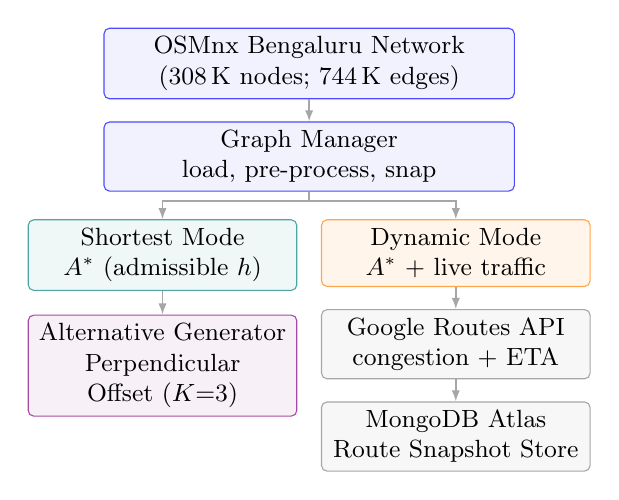
\begin{tikzpicture}[node distance=0.30cm and 0.35cm]
  \node[netbox] (osm) {OSMnx Bengaluru Network\\(308\,K nodes; 744\,K edges)};
  \node[netbox, below=0.28cm of osm] (gm) {Graph Manager\\load, pre-process, snap};

  \node[modeA, below left=0.35cm and 0.15cm of gm.south] (sh)
    {Shortest Mode\\$A^*$ (admissible $h$)};
  \node[modeB, below right=0.35cm and 0.15cm of gm.south] (dyn)
    {Dynamic Mode\\$A^*$ + live traffic};

  \node[altbox, below=0.30cm of sh] (off)
    {Alternative Generator\\Perpendicular Offset ($K{=}3$)};
  \node[extbox, below=0.28cm of dyn] (gapi)
    {Google Routes API\\congestion + ETA};
  \node[extbox, below=0.28cm of gapi] (mdb)
    {MongoDB Atlas\\Route Snapshot Store};

  \draw[arr] (osm) -- (gm);
  \draw[arr] (gm.south) -- ++(0,-0.12) -| (sh.north);
  \draw[arr] (gm.south) -- ++(0,-0.12) -| (dyn.north);
  \draw[arr] (sh)  -- (off);
  \draw[arr] (dyn) -- (gapi);
  \draw[arr] (gapi) -- (mdb);
\end{tikzpicture}
\caption{System architecture. GraphManager loads the Bengaluru road network. Shortest mode runs state-expanded $A^*$. Dynamic mode incorporates Google Routes API congestion polylines, re-computes $A^*$, and samples via-waypoints for traffic-aware ETAs. The alternative generator wraps the core search engine.}
\label{fig:architecture}
\end{figure}

The framework operates on a directed OpenStreetMap network of Bengaluru (308,643 vertices; 744,216 raw edges; 740,822 distinct ordered pairs after parallel-edge minimum-cost collapse).

\noindent\textbf{Shortest Mode} executes the turn-aware state-expanded $A^*$ search \cite{anirudhr2026turnaware} using road-class impedance and geometric turn penalties without live-traffic inputs.

\noindent\textbf{Dynamic Mode} retrieves real-time traffic polylines from the Google Routes API (TWO\_WHEELER travel mode, TRAFFIC\_AWARE preference).
Vertices along congested segments receive elevated traversal penalties, prompting $A^*$ to route around bottlenecks.
Upon path determination, Dynamic mode transmits up to 20 sampled via-waypoints along the calculated path back to the API to retrieve a traffic-aware ETA.

\textit{Independence note:} Because Dynamic mode ETAs are generated by querying Google Routes API using the framework's own route geometry, the framework and Google are not independent duration estimators. Their ETAs cannot be compared as competing measurements.

\noindent\textbf{Route Snapshot Logging:} In Dynamic mode, route geometry, distance, congested-node counts, and ETAs are persisted to MongoDB Atlas.

\subsection{Routing Cost Model}

The state-expanded $A^*$ model is detailed in the companion paper \cite{anirudhr2026turnaware}.
Each search state $s = (u, v)$ represents directed edge traversal, facilitating angular turn evaluation at vertex $v$.
The cost of transitioning from state $(u,v)$ to $(v,w)$ is:
\begin{equation}
  c\bigl((u,v)\to(v,w)\bigr) = c_\mu(v,w) + P_\text{turn}(u,v,w)
  \label{eq:astar_cost}
\end{equation}
where $c_\mu(v,w) = \ell(v,w)\cdot\mu(v,w)$ denotes impedance-weighted edge cost ($\ell$ is physical length in meters; $\mu$ is the road-class penalty multiplier).
The turn penalty $P_\text{turn}$ adds 25.0~m for angles $\ge 60^\circ$, 8.0~m for $30^\circ$--$60^\circ$, and 0.0~m otherwise \cite{anirudhr2026turnaware}.
The admissible heuristic function is:
\begin{equation}
  h(v) = 0.80 \cdot d_\text{Haversine}(v,\, t)
  \label{eq:heuristic}
\end{equation}
which is consistent under the verified network-wide bound $\mu(e) \ge 0.80$.

In Dynamic mode, congested vertices identified from traffic polylines incur a multiplied traversal penalty:
\begin{equation}
  \mu_\text{cong}(e) = 25 \cdot \mu(e), \quad u \in \mathcal{C} \text{ or } v \in \mathcal{C}
  \label{eq:congestion}
\end{equation}
where $\mathcal{C}$ denotes the set of congested network nodes.

\subsection{Perpendicular-Offset Waypoint Generation}

For origin $O=(\varphi_O,\lambda_O)$ and destination $D=(\varphi_D,\lambda_D)$ in decimal degrees, the forward azimuth of the chord is:
\begin{equation}
  \beta = \arctan2\!\left(\sin\Delta\lambda\cos\varphi_D,\;
         \cos\varphi_O\sin\varphi_D - \sin\varphi_O\cos\varphi_D\cos\Delta\lambda\right) \bmod 360^\circ
  \label{eq:bearing}
\end{equation}

At each chord fraction $\alpha \in \{0.33, 0.50, 0.67\}$, an intermediate base point is determined via linear interpolation:
\begin{equation}
  p_b(\alpha) = \bigl(\varphi_O + \alpha(\varphi_D-\varphi_O),\;\lambda_O + \alpha(\lambda_D-\lambda_O)\bigr)
  \label{eq:chord_point}
\end{equation}

Base points are laterally displaced using spherical destination-point equations.
For perpendicular directions $\beta_\perp \in \{\beta{+}90^\circ,\;\beta{-}90^\circ\}$ and lateral distances $d \in \{150~\text{m}, 300~\text{m}\}$:
\begin{align}
  \varphi_w &= \arcsin\!\left(\sin\varphi_b\cos\tfrac{d}{R} + \cos\varphi_b\sin\tfrac{d}{R}\cos\beta_\perp\right) \label{eq:dest_lat}\\
  \lambda_w &= \lambda_b + \arctan2\!\left(\sin\beta_\perp\sin\tfrac{d}{R}\cos\varphi_b,\;
              \cos\tfrac{d}{R}-\sin\varphi_b\sin\varphi_w\right) \label{eq:dest_lng}
\end{align}
where $R = 6{,}371{,}000$~m.
The resulting $3\times2\times2 = 12$ waypoints are snapped to the nearest network vertices, and duplicate vertices are removed.

\subsection{Candidate Route Generation and Filtering}

For each distinct offset vertex $w$, a two-leg route candidate $P_w = (O\to w)\oplus(w\to D)$ is stitched from two independent $A^*$ executions.
Candidates pass through four sequential filters:

(1)~\textit{Connectivity check}: $P_w$ must form a continuous graph path.

(2)~\textit{Duplicate suppression}: $P_w$ is discarded if its vertex sequence matches the primary route $P_0$ or any previously accepted alternative.

(3)~\textit{Detour constraint}: the physical distance ratio $\varepsilon$ must satisfy:
\begin{equation}
  \varepsilon(P_w) = \frac{\mathrm{dist}(P_w)}{\mathrm{dist}(P_0)} \;\le\; \varepsilon_{\max} = 1.20
  \label{eq:detour}
\end{equation}
where $\mathrm{dist}(P) = \sum_{e\in P} \ell(e)$ sums physical edge lengths in meters.

(4)~\textit{Edge-overlap constraint}: the physical length overlap $\gamma$ against the primary path must satisfy:
\begin{equation}
  \gamma(P_w, P_0) = \frac{\sum_{e\,\in\, E(P_w)\cap E(P_0)}\ell(e)}{\sum_{e\,\in\, E(P_w)}\ell(e)} \;\le\; \gamma_{\max} = 0.70
  \label{eq:overlap}
\end{equation}

Survivors are sorted in ascending order of impedance cost, and the top $K=3$ alternatives are retained.

\subsection{Route Diversity Metric}

Length-weighted Jaccard edge-set similarity between two routes $P_i$ and $P_j$ is defined as:
\begin{equation}
  J(P_i, P_j) = \frac{\sum_{e\in E(P_i)\cap E(P_j)}\ell(e)}{\sum_{e\in E(P_i)\cup E(P_j)}\ell(e)}
  \label{eq:jaccard}
\end{equation}
where union length equals $\mathrm{dist}(P_i) + \mathrm{dist}(P_j) - \sum_\cap\ell(e)$.
Pairwise diversity $\mathcal{D}$ across all returned paths (primary plus alternatives) is:
\begin{equation}
  \mathcal{D} = 1 - \frac{1}{|\mathcal{P}|}\sum_{i < j} J(P_i, P_j), \quad \mathcal{P} = \binom{\text{all routes}}{2}
  \label{eq:diversity}
\end{equation}

\subsection{Dynamic Routing and Congestion Integration}

Dynamic mode applies Eq.~(\ref{eq:congestion}) to avoid live traffic congestion identified via Google Routes API polylines.
The re-calculated path is then sampled at up to 20 uniform via-waypoints to retrieve a traffic-aware ETA.
The alternative-route module executes on the Shortest-mode engine without live-traffic inputs, matching the evaluation setup of Experiment E.

\begin{algorithm}[t]
\small
\caption{Perpendicular-Offset Alternative Route Generation}
\label{alg:offset}
\begin{algorithmic}[1]
\Require Graph $G=(V,E)$, origin $O$, destination $D$, primary route $P_0$
\Require $F=\{0.33,0.50,0.67\}$, $\Delta=\{150,300\}$~m, $\varepsilon_{\max}=1.20$, $\gamma_{\max}=0.70$, $K=3$
\Ensure Set $A$ of alternative routes, $|A|\le K$
\State $\beta \leftarrow \text{ForwardBearing}(O, D)$ \Comment{Eq.~\ref{eq:bearing}}
\State $W \leftarrow \emptyset$
\For{$\alpha \in F$}
  \State $p_b \leftarrow \text{ChordPoint}(O, D, \alpha)$ \Comment{Eq.~\ref{eq:chord_point}}
  \For{$d \in \Delta$}
    \For{$\beta_\perp \in \{\beta{+}90^\circ, \beta{-}90^\circ\}$}
      \State $w \leftarrow \text{DestinationPoint}(p_b, \beta_\perp, d)$ \Comment{Eqs.~\ref{eq:dest_lat}--\ref{eq:dest_lng}}
      \State $W \leftarrow W \cup \{\text{NearestNode}(G, w)\}$
    \EndFor
  \EndFor
\EndFor
\State $W \leftarrow \text{DeduplicateNodes}(W)$
\State $\mathit{seen} \leftarrow \{\text{NodeSeq}(P_0)\}$; $\;A \leftarrow \emptyset$; $\;\mathit{Surv} \leftarrow \emptyset$
\For{$w \in W$}
  \State $P_w \leftarrow \text{AStar}(O,w) \oplus \text{AStar}(w,D)$
  \State \textbf{if} $P_w \text{ is not connected}$ \textbf{then continue}
  \State \textbf{if} $\text{NodeSeq}(P_w) \in \mathit{seen}$ \textbf{then continue}
  \State $\mathit{seen} \leftarrow \mathit{seen} \cup \{\text{NodeSeq}(P_w)\}$
  \State \textbf{if} $\varepsilon(P_w) > \varepsilon_{\max}$ \textbf{then continue} \Comment{Eq.~\ref{eq:detour}}
  \State \textbf{if} $\gamma(P_w, P_0) > \gamma_{\max}$ \textbf{then continue} \Comment{Eq.~\ref{eq:overlap}}
  \State $\mathit{Surv} \leftarrow \mathit{Surv} \cup \{P_w\}$
\EndFor
\State Sort $\mathit{Surv}$ by ascending impedance cost; $A \leftarrow \mathit{Surv}_{1:\min(K,|\mathit{Surv}|)}$
\State \Return $A$
\end{algorithmic}
\end{algorithm}

% ============================================================
% IV. EVALUATION METHODOLOGY
% ============================================================

\section{Evaluation Methodology}

\subsection{Experiment E: Alternative-Route Evaluation}
\label{sec:methE}

Experiment E evaluates the offset method (E1) on 25 Bengaluru origin-destination corridors from the companion study \cite{anirudhr2026turnaware}.
Corridors span 1.4 to 15.0~km across three length categories: Short ($<5$~km, $n=7$), Medium (5--10~km, $n=10$), and Long ($>10$~km, $n=8$).
Execution time is the median of three consecutive runs using \texttt{time.perf\_counter()}; metrics are extracted directly from the frozen ablation dataset.

A five-corridor subset (OD\_01, OD\_02, OD\_03, OD\_04, OD\_23) compares E1 against Raw Yen (E2) and Filtered Yen (E3, which applies identical detour and overlap filters to Yen paths).
This five-corridor subset includes two corridors where E1 yields zero alternatives (OD\_04 and OD\_23) and is \textbf{descriptive only}.
At $n=5$, the minimum two-sided Wilcoxon $p$-value is 0.0625; no statistical significance is claimed.

All counts, means, medians, and execution times are \textbf{Measured} from original ablation JSON records.
The total count of candidates rejected by overlap filtering under E3 is 323 (\textbf{Measured}).

\subsection{Pilot External Comparison}
\label{sec:methPilot}

A descriptive pilot evaluated the framework, Google Maps (motorcycle tab, ``Leave now''), and Waze (motorcycle mode, user-confirmed) across four anonymised pairs (Pair~A to Pair~D), disjoint from the Experiment E corpus.
Queries were executed within approximately 10 minutes per pair during a single weekday evening window.
Primary route distance and estimated travel time were transcribed directly from visual map interfaces (\textbf{Measured}).
Waze motorcycle vehicle configuration is \textbf{User-confirmed}.
Collection timing is \textbf{Unverified} (inferred from timestamps).

Dynamic mode ETAs rely on sampled waypoints submitted to Google Routes API; the framework and Google are therefore not independent estimators.
No physical travel was conducted on pilot pairs, and no platform ranking is asserted.

\subsection{Strava Journey Analysis}
\label{sec:methStrava}

Five GPS trajectories between two fixed endpoints (Point~1 and Point~2) were collected over three days (Day~1 to Day~3, AM and PM), with morning trips running Point~1~$\to$~Point~2 and afternoon trips reversed.
Distances were calculated via Haversine summation ($R = 6{,}371{,}008.8$~m) from GPX logs; elapsed time represents the difference between final and initial timestamps.
Speed below $0.50$~m/s is classified as stopped; static intervals exceeding 5~s are recorded as tracking gaps.
Spatial deviation between repeated rides was computed via nearest-polyline distances, excluding non-overlapping endpoints.

All distance, duration, velocity, and consistency metrics are \textbf{Measured}.
Raw GPX files are preserved in the author's private archive.
Recorded Strava activity categories differ from the two-wheeler vehicle used.
Elapsed journey times (28.4--34.8~min) reflect physical traffic conditions and cannot be compared against algorithmic ETAs.

% ============================================================
% V. RESULTS
% ============================================================

\section{Results}

\subsection{Experiment E: Alternative-Route Generation}

\begin{figure*}[t]
\centering
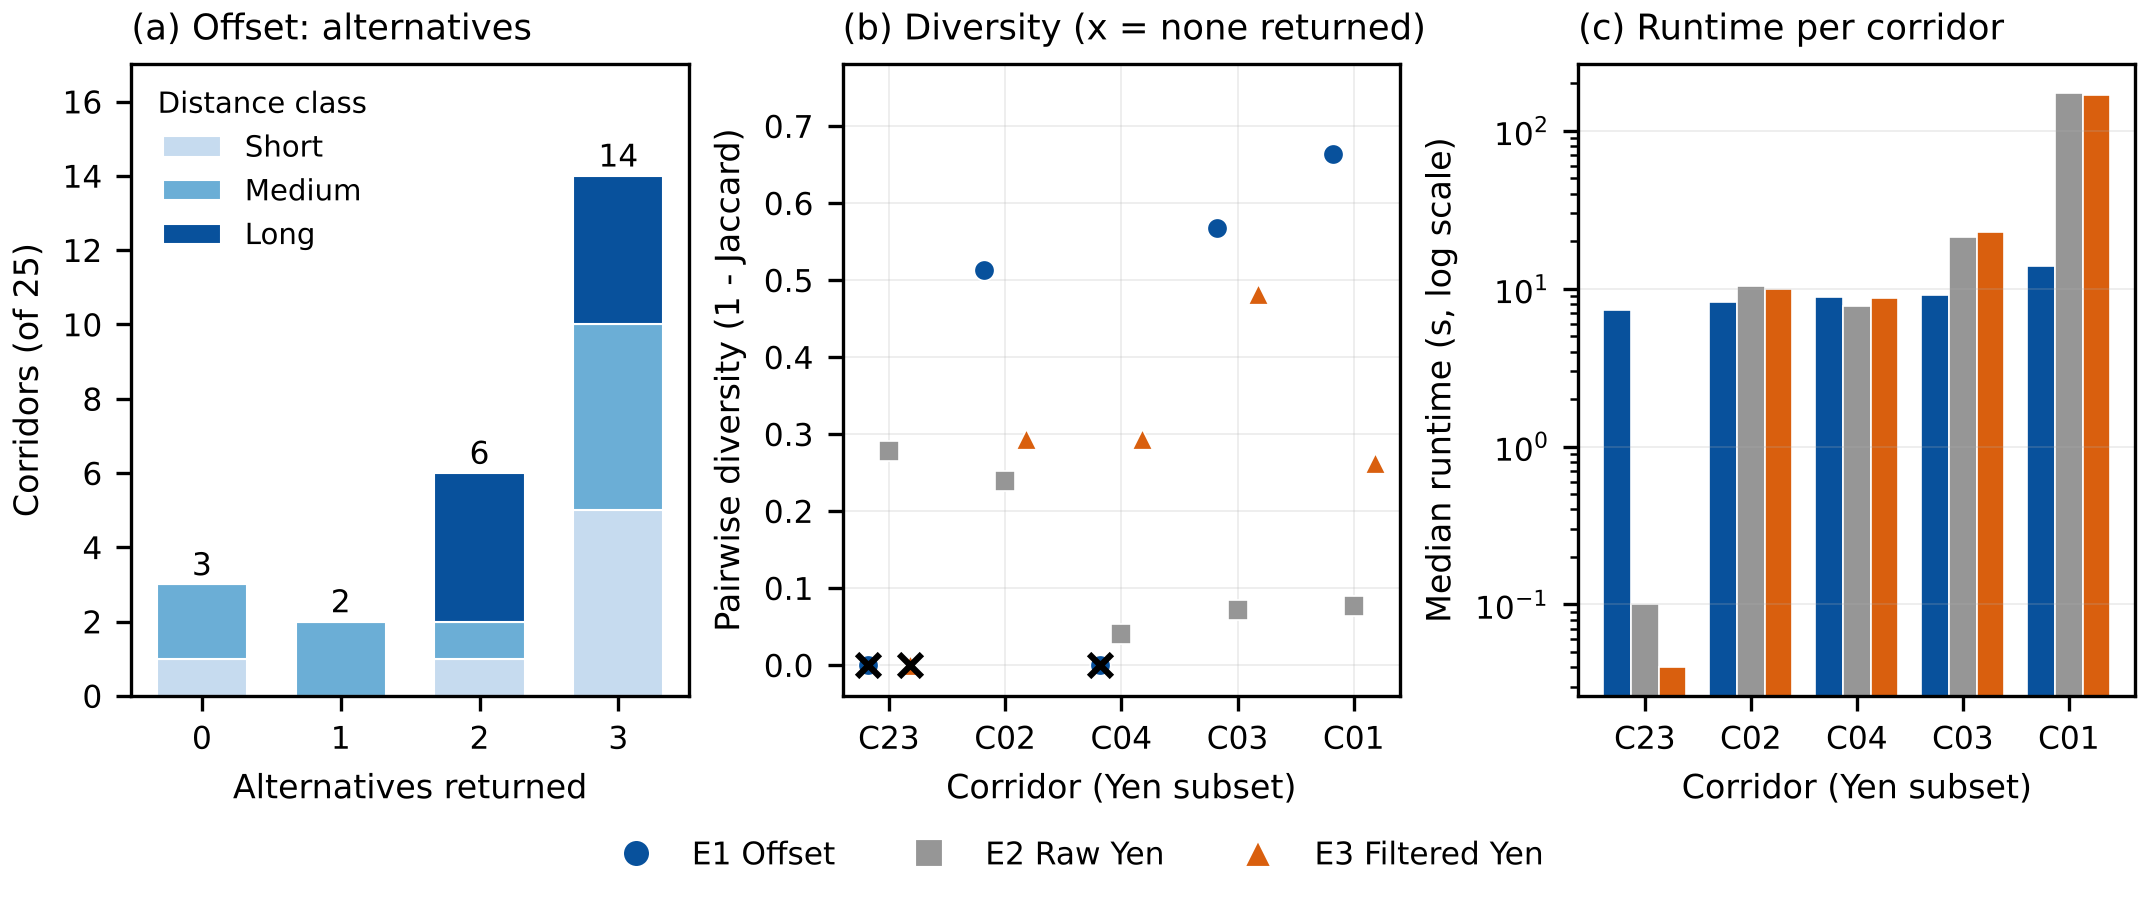
\includegraphics[width=0.96\textwidth]{fig_expE_phase3.png}
\caption{Experiment E evaluation across E1 (Perpendicular Offset, $N=25$), E2 (Raw Yen, $N=5$), and E3 (Filtered Yen, $N=5$). E1 spans all 25 corridors; E2 and E3 evaluate the five-corridor subset. Execution times for E2 and E3 are dominated by OD\_01 (173.6~s and 169.6~s, respectively) and are descriptive.}
\label{fig:expE}
\end{figure*}

\begin{table}[t]
\caption{Experiment E1: Offset Method across 25 Corridors (Measured)}
\label{tab:expE_offset}
\centering
\footnotesize
\setlength{\tabcolsep}{2pt}
\renewcommand{\arraystretch}{1.08}
\begin{tabular}{@{}lrrrrr@{}}
\hline
\textbf{Class} & \textbf{$n$} & \textbf{Any alt.} & \textbf{K=3} & \textbf{Mean alts.} & \textbf{Div.} \\
\hline
Short           & 7  & 6 (85.7\%) & 5 & 2.43 & 0.622 \\
Medium          & 10 & 8 (80.0\%) & 5 & 1.90 & 0.530 \\
Long            & 8  & 8 (100\%)  & 4 & 2.50 & 0.545 \\
\hline
\textbf{All}   & \textbf{25} & \textbf{22 (88.0\%)} & \textbf{14 (56.0\%)} & \textbf{2.24} & \textbf{0.561} \\
\hline
\end{tabular}
\vspace{2pt}
\begin{minipage}{\columnwidth}
\scriptsize
\textit{Notes:} Div.: mean pairwise diversity $\mathcal{D}$ (Eq.~\ref{eq:diversity}) on successful corridors ($\ge 1$ alternative); zero-padded mean across all 25 corridors is 0.4932. Runtime: median 9.09~s, mean 10.52~s, range 7.36--22.54~s. Mean detour 1.046; mean overlap 0.496 (56 alternatives). Three corridors (OD\_04, OD\_15, OD\_23) returned zero alternatives.
\end{minipage}
\end{table}

\noindent\textbf{Offset method (E1, 25 corridors):}
The offset generator produced valid alternatives on 22 of 25 corridors (88.0\%), returning the full complement of $K=3$ alternatives on 14 corridors (56.0\%).
Surviving alternatives averaged 2.24 across all corridors and 2.55 across successful corridors.
Mean pairwise diversity $\mathcal{D}$ (Eq.~\ref{eq:diversity}) reached 0.5605 (median 0.5672) for successful corridors; including failures as zero yields 0.4932.
All 56 accepted alternatives adhered to production constraints: maximum detour 1.1939 ($\le 1.20$) and maximum overlap 0.6911 ($\le 0.70$).
Execution times ranged from 7.36 to 22.54~s (median 9.09~s).
The three zero-alternative corridors (OD\_04, OD\_15, OD\_23) had all 12 candidates rejected by the detour filter due to severe network bottlenecks.
Table~\ref{tab:expE_offset} breaks down results by corridor length.

\noindent\textbf{Five-corridor comparison ($n=5$, descriptive):}
Filtered Yen (E3) achieved higher route coverage than the offset method (E1) on the five-corridor subset, averaging 2.4 vs.\ 1.2 alternatives and reaching $K=3$ on 4 vs.\ 1 corridor.
However, where both methods succeeded (OD\_01, OD\_02, OD\_03; $n=3$), offset alternatives exhibited greater topological diversity (mean diversity 0.58 vs.\ 0.35) and lower overlap (mean 0.44 vs.\ 0.53).
Raw Yen (E2) reached $K=3$ across all five corridors but produced near-duplicate paths (mean overlap 0.93, diversity 0.13).
This demonstrates a coverage-versus-diversity trade-off: filtered Yen provides broader coverage, whereas the offset method yields higher spatial separation where feasible.
Mean runtimes were 9.5~s for E1, 42.6~s for E2, and 41.5~s for E3, heavily influenced by OD\_01.
Yen was faster on two corridors; no overall speed-up is claimed.
Under E3, 323 candidates were pruned by overlap filtering.

\subsection{Pilot External Comparison}

\begin{figure*}[t]
\centering
\begin{minipage}[t]{0.32\textwidth}
  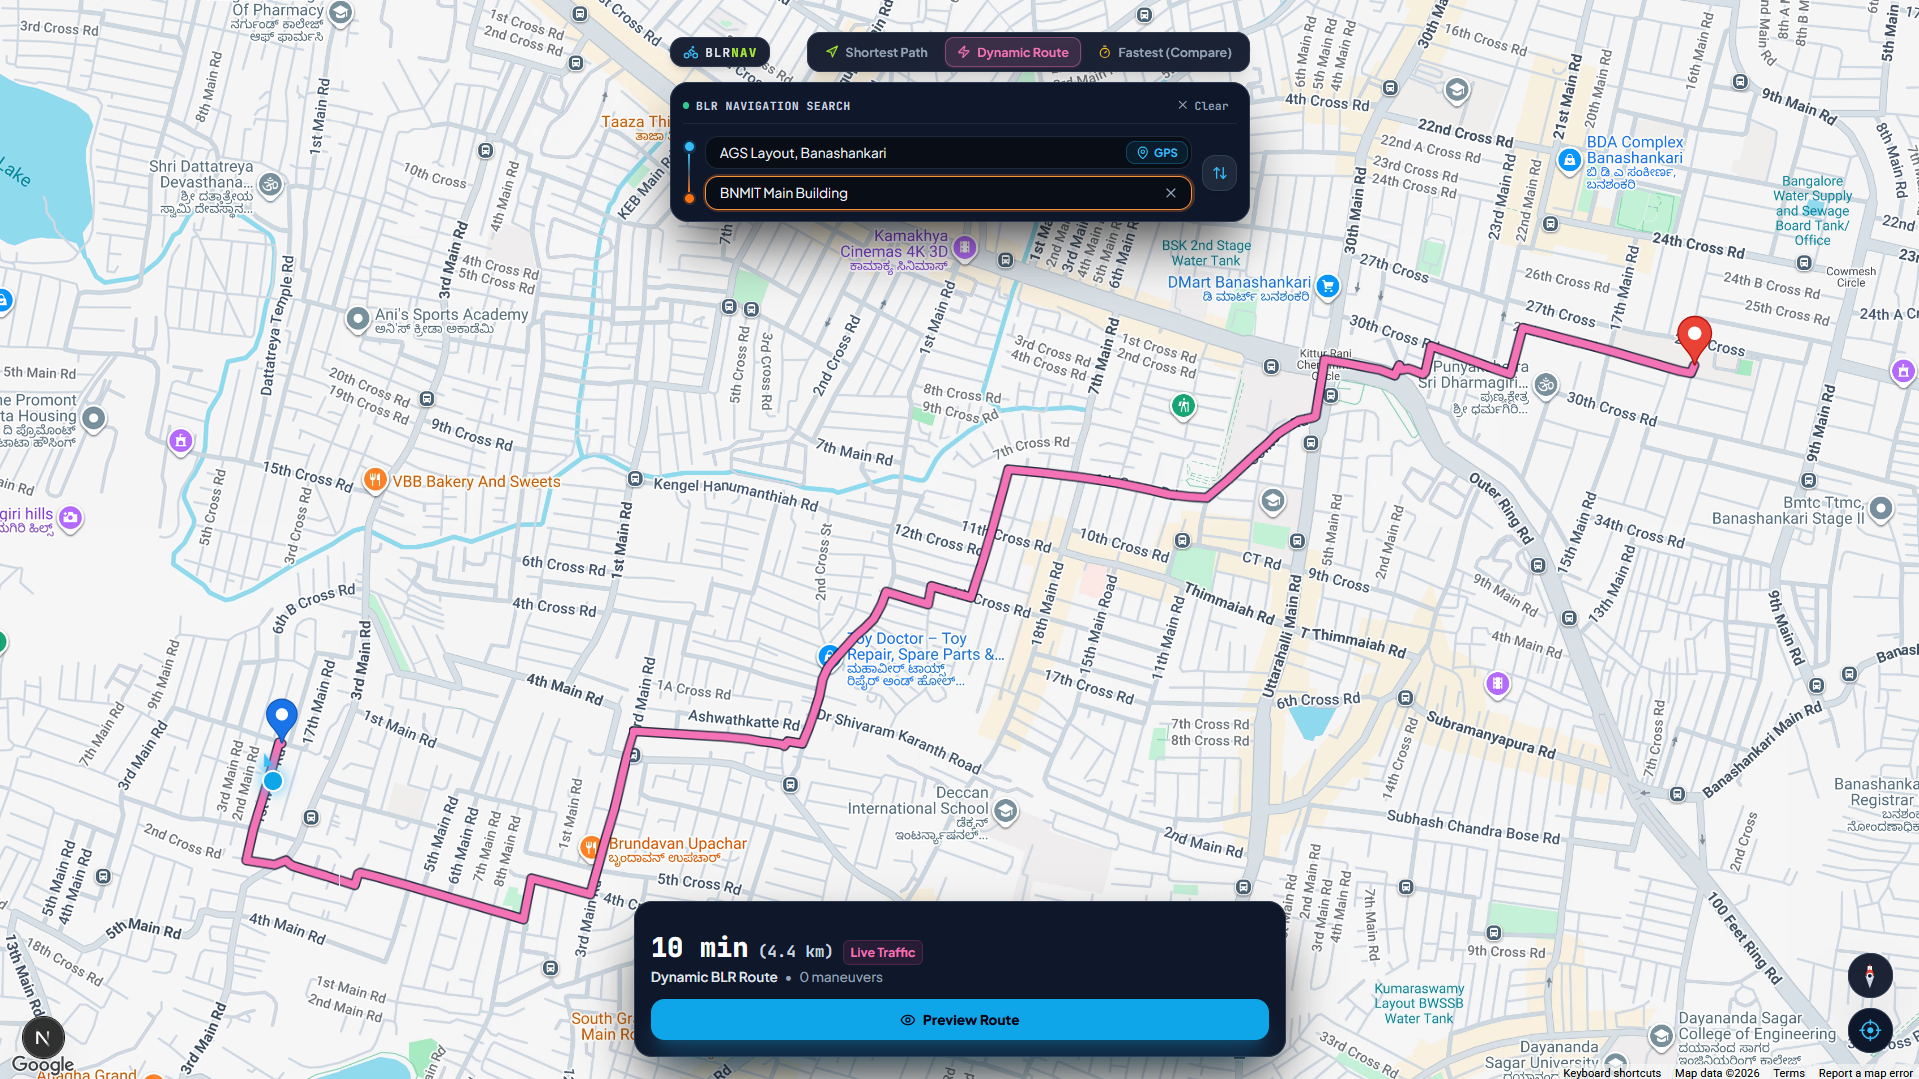
\includegraphics[width=\linewidth]{pair_b_project.png}
  \centerline{\footnotesize (a) Routing framework (Dynamic mode)}
\end{minipage}\hfill
\begin{minipage}[t]{0.32\textwidth}
  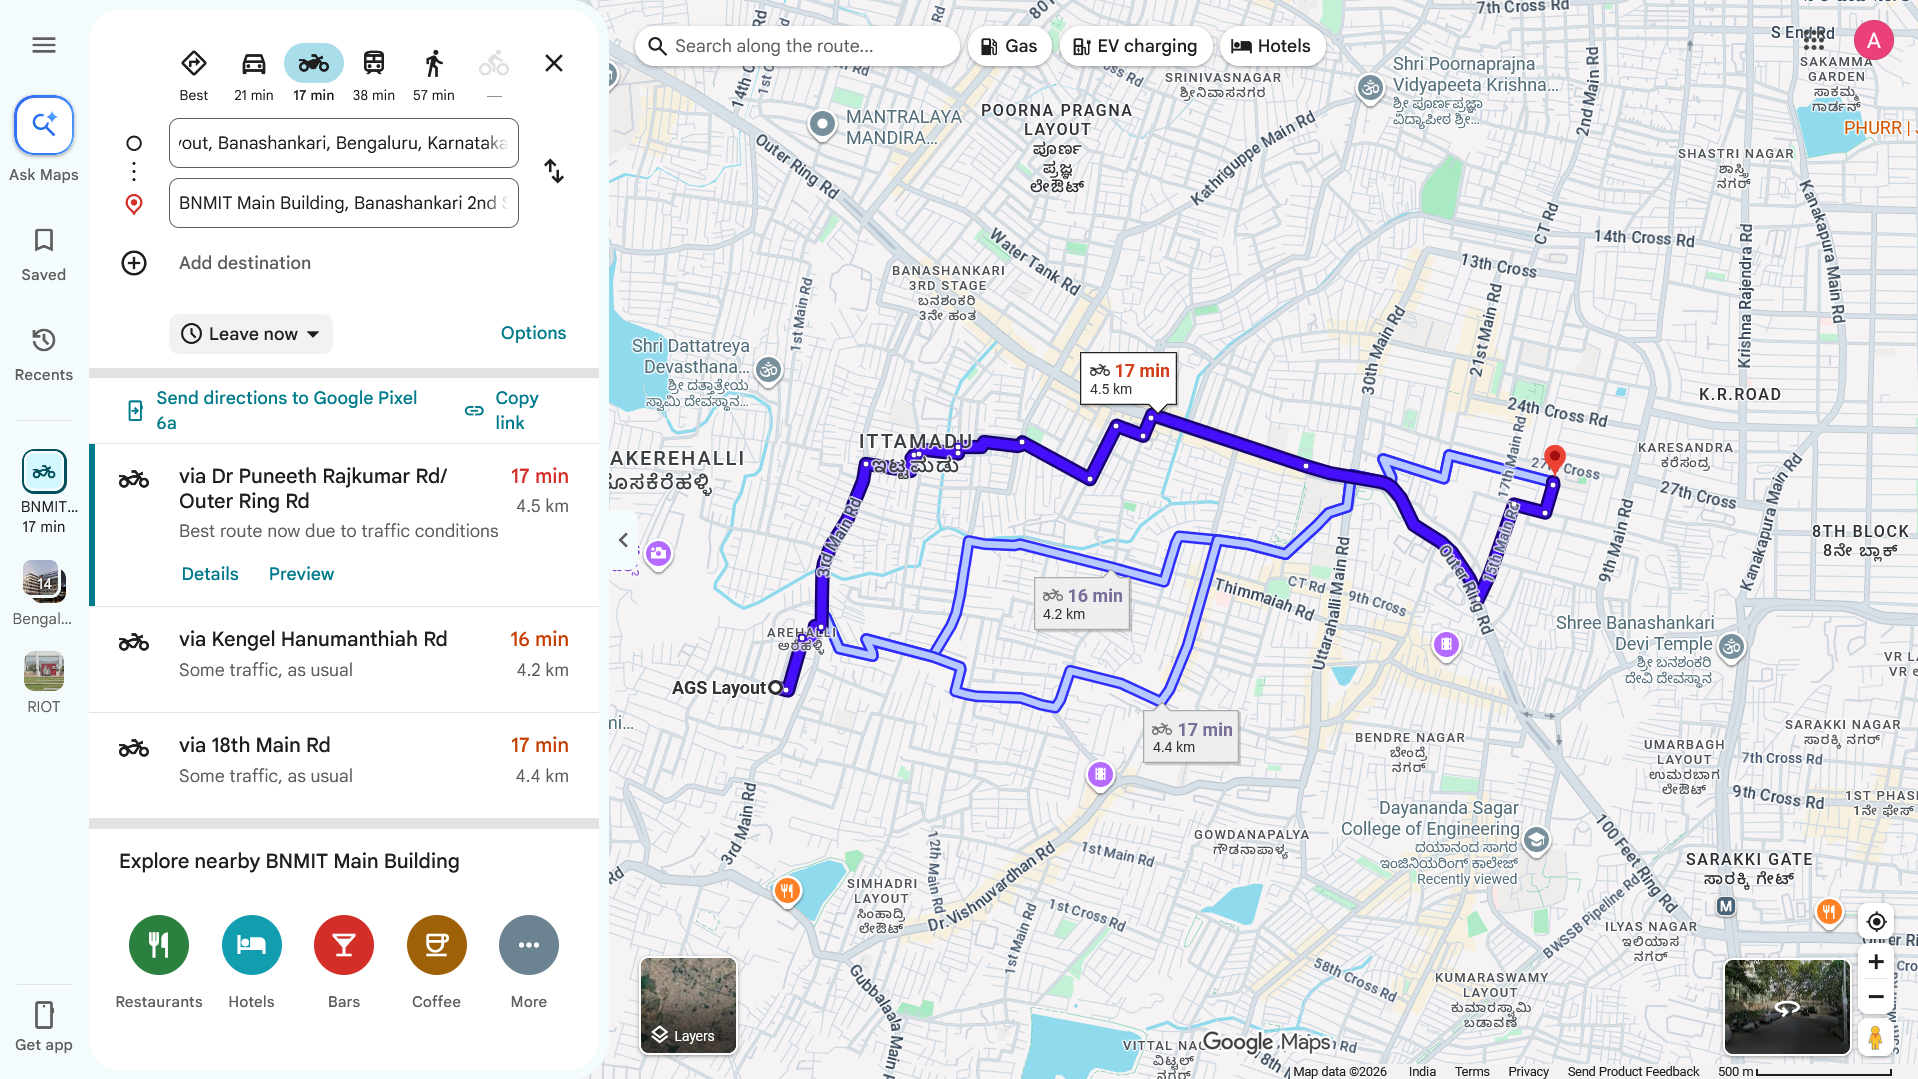
\includegraphics[width=\linewidth]{pair_b_gmaps.png}
  \centerline{\footnotesize (b) Google Maps (motorcycle tab)}
\end{minipage}\hfill
\begin{minipage}[t]{0.32\textwidth}
  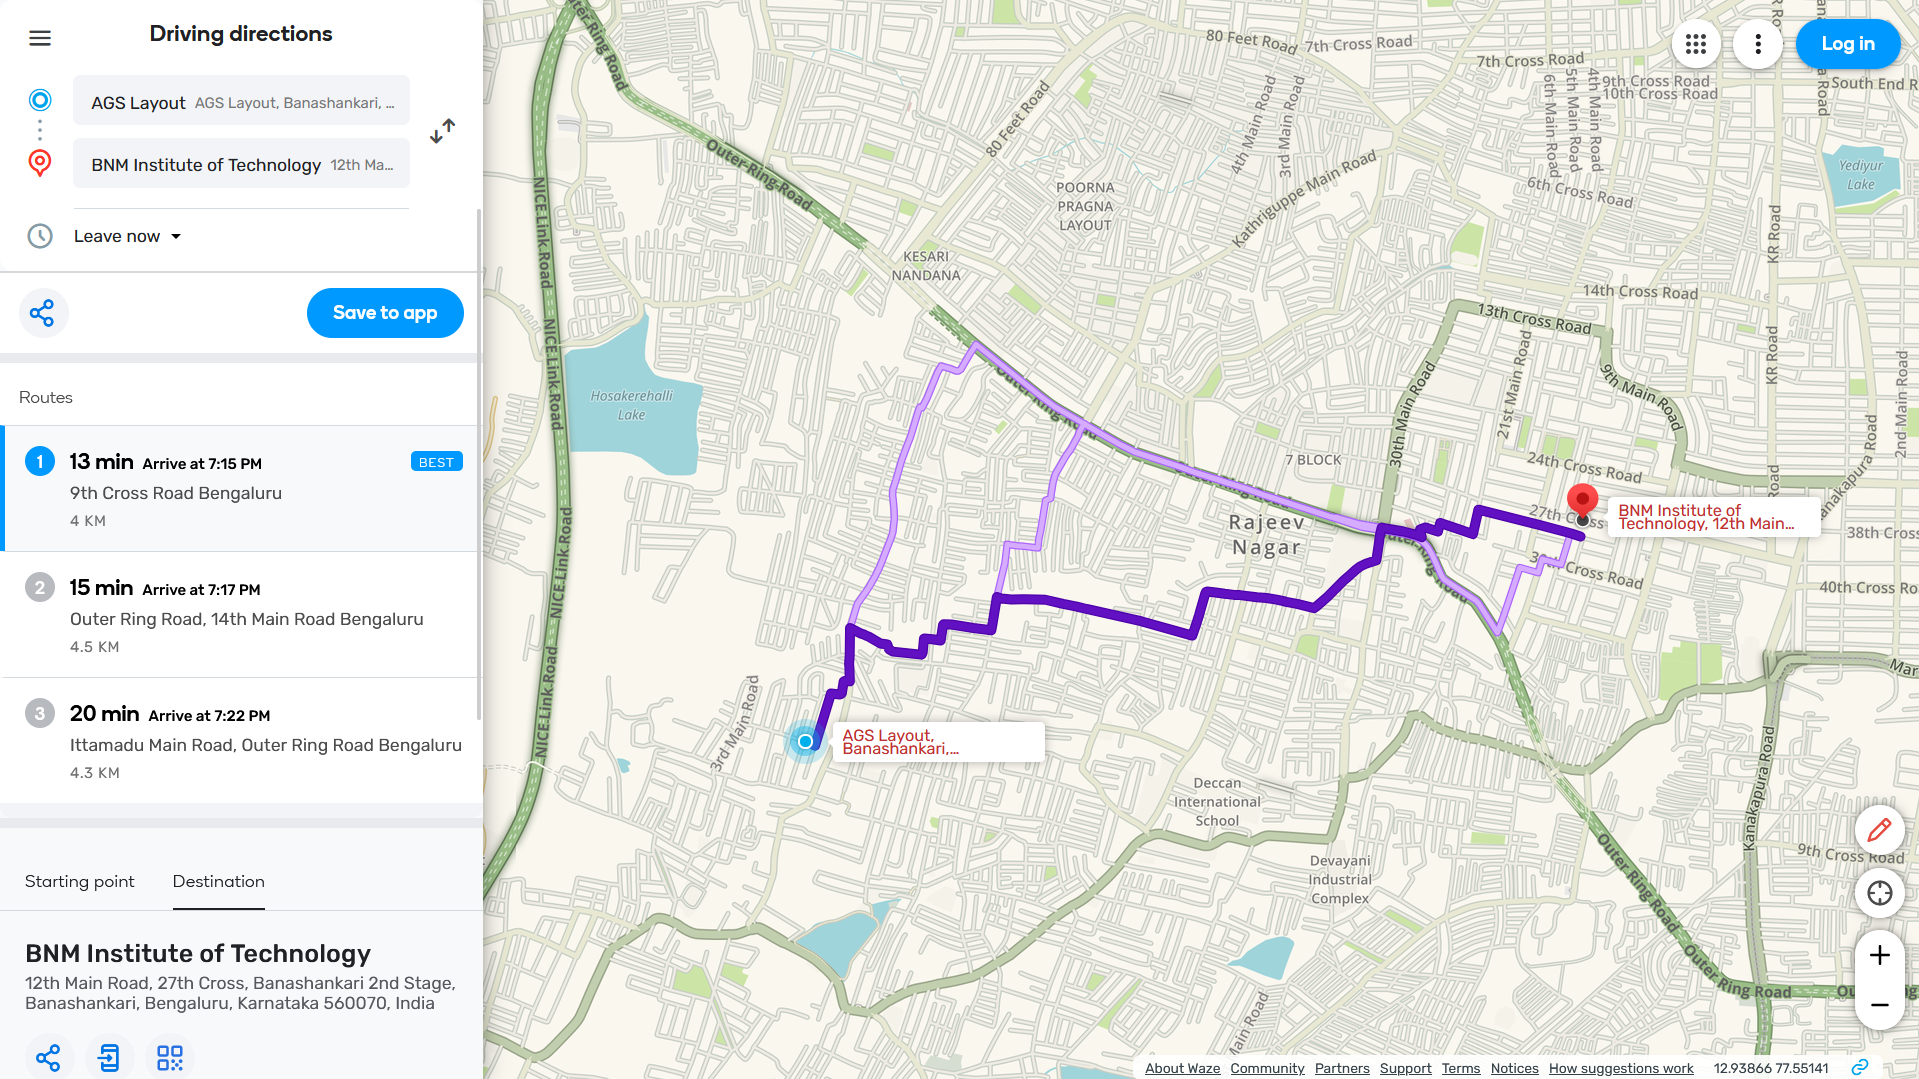
\includegraphics[width=\linewidth]{pair_b_waze.png}
  \centerline{\footnotesize (c) Waze (motorcycle vehicle type)}
\end{minipage}
\caption{Pilot Pair~B (Short class) visual interface captures: routing framework (Dynamic mode), Google Maps (motorcycle tab), and Waze (motorcycle type). Images display third-party map tiles and place names; precise coordinates remain confidential. The routing framework outputs a single route by design, whereas Google Maps and Waze present three alternatives.}
\label{fig:pilot_case}
\end{figure*}

\begin{table}[t]
\caption{Pilot Comparison: Pairs A to D (Measured from Screenshots)}
\label{tab:pilot}
\centering
\footnotesize
\setlength{\tabcolsep}{2pt}
\renewcommand{\arraystretch}{1.08}
\begin{tabular}{@{}lcrrrrrr@{}}
\hline
\textbf{Pair} & \textbf{Class} & \multicolumn{2}{c}{\textbf{Framework}} & \multicolumn{2}{c}{\textbf{Google Maps}} & \multicolumn{2}{c}{\textbf{Waze}} \\
 & & km & min & km & min & km & min \\
\hline
A & Long   & 24.2 & 53 & 33.7 & 65 & 21.7 & 62 \\
B & Short  &  4.4 & 10 &  4.5 & 17 &  4.0 & 13 \\
C & Long   & 17.4 & 59 & 15.6 & 65 & 14.6 & 75 \\
D & Medium & 13.2 & 41 & 16.8 & 52 & 17.4 & 55 \\
\hline
\end{tabular}
\vspace{2pt}
\begin{minipage}{\columnwidth}
\scriptsize
\textit{Notes:} Four pairs captured in one evening window. Waze motorcycle mode is user-confirmed. Framework ETAs are derived via Google Routes API via-waypoints (non-independent). Pair~A Waze route flagged toll usage. No physical travel was conducted; metrics are model predictions only.
\end{minipage}
\end{table}

Table~\ref{tab:pilot} displays predicted distances and travel times across Pairs A--D.
The framework returns one route per request by design; commercial platforms display multiple alternatives.
Values reflect divergent geocoding, base networks, and traffic feeds; they cannot be treated as equivalent measurements.
Because framework ETAs rely on Google Routes API queries, they share provenance with Google estimates.
No platform ranking or performance superiority is derived from this pilot.

\subsection{Strava Journey Analysis}

\begin{figure*}[t]
\centering
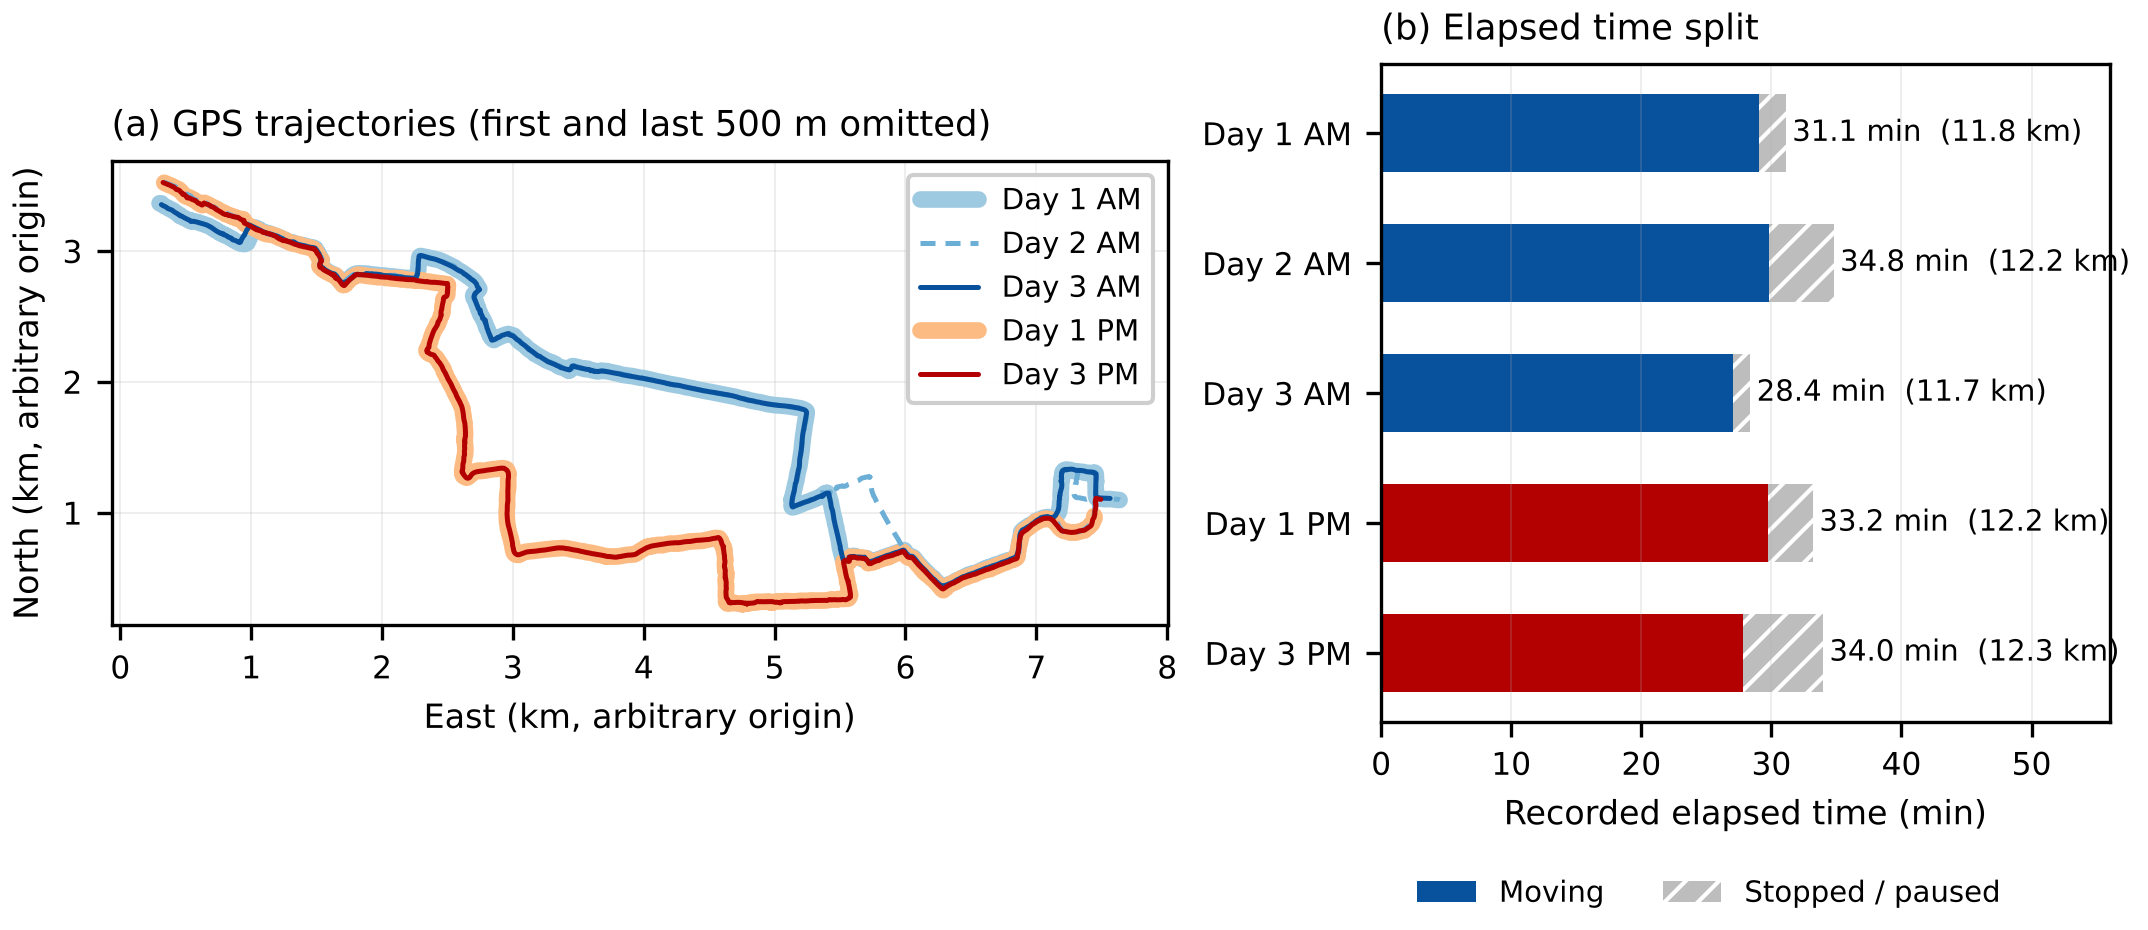
\includegraphics[width=0.96\textwidth]{fig_strava_phase2.png}
\caption{GPS trajectory analysis across five rides on three days. Top: anonymised trajectories in arbitrary-origin meters with the first and last 500~m excluded; morning (AM) and afternoon (PM) rides displayed separately. Bottom: stacked time breakdown (moving vs.\ stopped, threshold 0.50~m/s) per ride. Coordinates and timestamps are removed; raw GPX files remain in the author's private archive.}
\label{fig:strava}
\end{figure*}

\begin{table}[t]
\caption{Strava Ride Summary: Five Rides Across Three Days (Measured from GPX)}
\label{tab:strava}
\centering
\footnotesize
\setlength{\tabcolsep}{2pt}
\renewcommand{\arraystretch}{1.08}
\begin{tabular}{@{}lrrrrr@{}}
\hline
\textbf{Ride} & \textbf{Dist.\ (km)} & \textbf{Elapsed (min)} & \textbf{Moving (min)} & \textbf{Stopped (min)} & \textbf{Stops} \\
\hline
Day 1 AM & 11.84 & 31.1 & 29.1 & 2.1 & 23 \\
Day 2 AM & 12.19 & 34.8 & 29.9 & 4.9 & 26 \\
Day 3 AM & 11.69 & 28.4 & 27.0 & 1.4 & 13 \\
Day 1 PM & 12.20 & 33.2 & 29.7 & 3.5 & 23 \\
Day 3 PM & 12.29 & 34.0 & 27.8 & 6.1 & 21 \\
\hline
\end{tabular}
\vspace{2pt}
\begin{minipage}{\columnwidth}
\scriptsize
\textit{Notes:} Stopped threshold: 0.50~m/s. Recording start and end locations varied slightly across rides; raw lengths are not directly comparable. Vehicle: two-wheeler. Elapsed times reflect traffic and cannot be compared against model ETAs. Stopped durations vary by 0.5--2.3~min across threshold sensitivity range (0.30--1.00~m/s).
\end{minipage}
\end{table}

Table~\ref{tab:strava} summarizes ride metrics, and Fig.~\ref{fig:strava} displays anonymised spatial trajectories and temporal breakdowns.
Morning journeys on Day~1 and Day~3 followed nearly identical routes: mean deviation was 3.4~m, P90 was 6.2~m, maximum was 50.9~m, and 98.1\% of tracking points lay within 15~m (\textbf{Measured}).
Afternoon journeys on Day~1 and Day~3 exhibited similar consistency: mean deviation was 2.9~m, P90 was 6.2~m, maximum was 18.6~m, and 99.8\% of points lay within 15~m (\textbf{Measured}).
The Day~2 morning journey diverged noticeably from the Day~1 and Day~3 trajectory: mean deviation was approximately 59~m, P90 reached 215~m, maximum was 443~m, and 68.2\% of points lay within 15~m.
The cause of this deviation is unknown.
A cross-comparison between Day~1 morning and afternoon paths yielded a mean divergence of 377~m, verifying that the metric clearly distinguishes separate corridors.
The afternoon trajectory was recommended by the framework following a real-time rerouting event and executed on Day~1 and Day~3 (\textbf{User-confirmed}).
The morning baseline route represents a \textbf{Recovered historical snapshot}; contemporaneous display was not independently validated.

% ============================================================
% VI. DISCUSSION AND LIMITATIONS
% ============================================================

\section{Discussion and Limitations}

\noindent\textbf{Alternative-Route Coverage and Diversity:}
The offset method achieves an 88.0\% corridor success rate, demonstrating that lateral waypoint displacement effectively identifies viable alternatives across typical urban layouts.
On corridors with severe topological barriers (such as OD\_04, OD\_15, and OD\_23), lateral excursions consistently exceed the 1.20 detour limit, returning no valid alternative.
Filtered Yen circumvents this geometric constraint by traversing the global shortest-path tree, albeit at the cost of higher edge overlap and lower spatial separation.
The five-corridor subset ($n=5$) illustrates this trade-off but remains purely descriptive.

\noindent\textbf{Pilot Comparison Scope and Platform Independence:}
The pilot study is restricted to four corridor pairs evaluated within a single evening window.
Commercial platforms rely on distinct road networks, proprietary geocoding, and independent traffic inputs.
Because framework ETAs are generated by querying the Google Routes API with framework path waypoints, the two services are not independent estimators.
Waze motorcycle settings are user-confirmed and not visible in archived screenshots.
These pilot observations document operational feasibility but do not establish platform rankings or travel-time superiority.

\noindent\textbf{Journey Analysis Scope:}
The empirical GPS corpus represents a single rider across three days on one origin-destination pair.
Variations in trip start and end locations preclude raw distance comparisons.
Total elapsed times (28.4--34.8~min) reflect traffic delays, signal stops, and rider behavior; they cannot validate algorithmic ETAs.
Stopped-time classifications are sensitive to velocity thresholds, shifting by 0.5--2.3~min across the 0.30--1.00~m/s range.
No definitive cause for the Day~2 morning detour can be confirmed.

\noindent\textbf{General Limitations and Future Work:}
Network analysis is restricted to a static OpenStreetMap snapshot of Bengaluru; unmapped infrastructure or subsequent modifications are omitted.
Turn deflection angles are derived from street centerline vectors and do not capture dynamic police diversions or temporary blockages.
Graph traversal impedance serves as a search cost rather than a calibrated measure of physical duration or energy consumption.
The signal-delay discount formulation present in experimental stubs was uninvoked in production runs and is excluded from all reported results \cite{promraksa2022lane,abbas2019internet}.
Future research will investigate multi-city generalisation, real-time dynamic graph updates, rider preference calibration, and IoT traffic sensing integration \cite{abbas2019internet}.

% ============================================================
% VII. CONCLUSION
% ============================================================

\section{Conclusion}

This paper presented and evaluated a two-wheeler routing framework extending a turn-aware state-expanded $A^*$ search engine \cite{anirudhr2026turnaware} with Shortest and Dynamic operational modes and a perpendicular-offset alternative-route generator.
Across 25 Bengaluru corridors, the offset generator produced valid alternatives ($\varepsilon \le 1.20$, $\gamma \le 0.70$) on 22 corridors (88.0\%), achieving an average pairwise diversity of 0.5605 on successful corridors.
A descriptive five-corridor benchmark against filtered Yen revealed a fundamental coverage-versus-diversity trade-off.
Manual pilot observations documented comparative platform metrics without asserting rankings, and repeat GPS journeys demonstrated spatial path consistency across multiple days.
No travel-time savings, safety improvements, or platform superiority are claimed; all findings constitute descriptive empirical measurements on an urban road network.

\balance
\bibliographystyle{IEEEtran}
\bibliography{paper2_verified_references}

\end{document}
